%% Supplementary material for the New Glenn explosion paper (FIRST DRAFT).
%% Compile:  latexmk -pdf NewGlenn_explosion_supplement.tex
\documentclass[11pt]{article}
\usepackage[margin=2.2cm]{geometry}
\usepackage{graphicx}
\usepackage{amsmath}
\usepackage{siunitx}
\usepackage{booktabs}
\usepackage[font=small]{caption}
\graphicspath{{figures/}}
\renewcommand{\thefigure}{S\arabic{figure}}
\renewcommand{\thetable}{S\arabic{table}}
\setlength{\parindent}{0pt}
% Shrink a table to the text width only when it is wider (tables/*.tex use this).
\newsavebox{\fitbox}
\newcommand{\fitwidth}[1]{\sbox{\fitbox}{#1}\ifdim\wd\fitbox>\textwidth\resizebox{\textwidth}{!}{\usebox{\fitbox}}\else\usebox{\fitbox}\fi}

\title{Supplementary material for\\ ``Seismo-acoustic recordings of the May~2026 New~Glenn static-fire explosion at Cape~Canaveral''}
\author{Glenn Thompson, Robert G. Brown, John Kiriazes, Paul Bremner, Han Byul Woo, Sue Bilek}
\date{}

\begin{document}
\maketitle

Tables S1--S14 and Figures S1--S7 support the main text. They were produced by the notebooks in
\texttt{10\_NewGlenn\_paper} (numbers in brackets); the tables are written by notebook 40 from the other
notebooks' output files.

\section*{Tables}

\begin{table}[htbp]
  \centering
  \caption{Stations recording on 29~May~2026: coordinates, distance and azimuth from LC-36 (28.4706$^\circ$N, 80.5422$^\circ$W), sampling rate and status for the explosion [21, 22].}
  \label{tab:s_stations}
  \small
  \fitwidth{%
\begin{tabular}{lrrrrrp{5.2cm}}
\toprule
Station & Lat ($^\circ$N) & Lon ($^\circ$E) & Distance (km) & Azimuth ($^\circ$) & Samples s$^{-1}$ & Status \\
\midrule
B20 & 28.5736 & -80.5722 & 11.79 & 345.6 & 100 & infraBSU HD1; Trillium (noisy; horizontals identical); Chaparral (clipped, faulty) \\
B24 & 28.5806 & -80.6408 & 15.55 & 321.6 & 500 & none (no sensors connected) \\
B01 & 28.6214 & -80.6067 & 17.87 & 339.3 & 500 & none (no sensors connected) \\
B14 & 28.6322 & -80.6158 & 19.31 & 338.1 & 500 & infraBSUs CD0, CD1, CD2; Trillium \\
B03 & 28.6428 & -80.6236 & 20.68 & 337.4 & 500 & none (no sensors; Centaur faulty) \\
B29 & 28.6181 & -80.6769 & 21.00 & 321.1 & 500 & infraBSU CD0; Trillium \\
B05 & 28.6400 & -80.6450 & 21.30 & 331.8 & 500 & infraBSU CD0; Trillium (CH2 at its stop) \\
\bottomrule
\end{tabular}
  }
\end{table}

\begin{table}[htbp]
  \centering
  \caption{Channel status for the explosion, with the pre-event noise in raw counts (rms, 250--20~s before the origin) in brackets [22]. ok: working; none: no sensor connected (digitizer noise only); rail: within 20\% of the 24-bit rail during the event (Trillium mass at its stop, or a clipped sensor); same: records the same signal as the other horizontal (B20 DH1 and DH2 correlate at 0.9999 all year). B03\textquoteright s Centaur channels are also known to be faulty.}
  \label{tab:s_channels}
  \scriptsize
  \fitwidth{%
\begin{tabular}{llllllll}
\toprule
Station & DHZ & DH1 & DH2 & DD0 & DD1 & DD2 & DDF \\
\midrule
B20 & ok (36,944) & same (12,644) & same (12,917) & -- & ok (344) & none (9.2) & rail (156,643) \\
B24 & none (2.4) & none (1.7) & none (1.8) & none (13.2) & none (13.4) & none (13.2) & -- \\
B01 & none (2.8) & none (1.9) & none (2.0) & none (13.8) & none (13.7) & none (13.6) & -- \\
B14 & ok (892) & ok (437) & ok (582) & ok (3,950) & ok (3,299) & ok (163) & -- \\
B03 & none (3.9) & none (2.0) & none (2.0) & none (17.4) & none (14.3) & none (14.9) & -- \\
B29 & ok (121) & ok (175) & ok (163) & ok (95.6) & none (14.5) & none (14.6) & -- \\
B05 & ok (104) & ok (193) & rail (353) & ok (8,758) & none (14.4) & none (14.7) & -- \\
\bottomrule
\end{tabular}
  }
\end{table}

\begin{table}[htbp]
  \centering
  \caption{Surface weather within 30~minutes of the origin (Iowa Environmental Mesonet ASOS; means of the observations): XMR, Cape Canaveral Skid Strip (2~km from LC-36); TTS, Shuttle Landing Facility (within the network); COF, Patrick Space Force Base (not used) [24].}
  \label{tab:s_weather}
  \small
  \fitwidth{%
\begin{tabular}{lrrrrrr}
\toprule
Station & Obs. & T ($^\circ$C) & RH (\%) & Pressure (hPa) & Wind (m~s$^{-1}$) & Wind from ($^\circ$) \\
\midrule
COF & 1 & 28.3 & 80.9 & 1014.0 & 5.1 & 290 \\
TTS & 8 & 25.8 & 88.8 & 1014.3 & 0.5 & 300 \\
XMR & 3 & 27.1 & 85.5 & 1013.6 & 3.9 & 297 \\
\bottomrule
\end{tabular}
  }
\end{table}

\begin{table}[htbp]
  \centering
  \caption{Predicted airwave speed to each working station: still-air speed $c_0$ (Cramer, 1993) for the mean of XMR and TTS (26.4~$^\circ$C, 87\% RH, 1014~hPa), the component of the mean wind along the source--station ray, the effective speed and the travel time [24].}
  \label{tab:s_speeds}
  \small
  \fitwidth{%
\begin{tabular}{lrrrrr}
\toprule
Station & Azimuth ($^\circ$) & $c_0$ (m~s$^{-1}$) & Wind along ray (m~s$^{-1}$) & $c_\mathrm{eff}$ (m~s$^{-1}$) & Travel time (s) \\
\midrule
B20 & 345.6 & 348.7 & -1.47 & 347.3 & 33.96 \\
B14 & 338.1 & 348.7 & -1.67 & 347.1 & 55.64 \\
B29 & 321.1 & 348.7 & -2.01 & 346.7 & 60.57 \\
B05 & 331.8 & 348.7 & -1.81 & 346.9 & 61.41 \\
\bottomrule
\end{tabular}
  }
\end{table}

\begin{table}[htbp]
  \centering
  \caption{Airwave onsets at the working infraBSUs, in seconds after the adopted origin (01:00:02.37~UTC): first sample above 5, 10 or 20\% of the peak, and never below five times the noise [24].}
  \label{tab:s_onsets}
  \small
  \fitwidth{%
\begin{tabular}{lrrrrrr}
\toprule
Channel & Distance (km) & Peak (Pa) & Noise (Pa) & Onset 5\% (s) & Onset 10\% (s) & Onset 20\% (s) \\
\midrule
B20.00.DD1 & 11.79 & 364 & 0.06 & 33.62 & 33.79 & 34.26 \\
B14.00.DD0 & 19.31 & 236 & 4.62 & 55.61 & 55.61 & 56.15 \\
B14.00.DD1 & 19.31 & 305 & 1.25 & 55.52 & 55.69 & 56.14 \\
B14.00.DD2 & 19.31 & 244 & 0.05 & 55.52 & 55.69 & 56.15 \\
B29.00.DD0 & 21.00 & 296 & 0.03 & 61.00 & 61.50 & 61.51 \\
B05.00.DD0 & 21.30 & 256 & 4.73 & 61.58 & 61.63 & 62.07 \\
\bottomrule
\end{tabular}
  }
\end{table}

\begin{table}[htbp]
  \centering
  \caption{Origin time for each onset definition and speed model: weather-based speed with the mean wind (adopted with the 5\% onsets), XMR weather only, no wind, and a straight-line fit with the speed free. Spread: standard deviation of the station origins; trend: their drift with distance [24].}
  \label{tab:s_origin}
  \small
  \fitwidth{%
\begin{tabular}{llrrrr}
\toprule
Onset & Model & Origin (UTC) & Speed (m~s$^{-1}$) & Spread (s) & Trend (s~km$^{-1}$) \\
\midrule
5\% & weather + wind & 01:00:02.37 & 347.0 & 0.27 & 0.059 \\
5\% & XMR only + wind & 01:00:02.22 & 346.1 & 0.22 & 0.047 \\
5\% & weather, no wind & 01:00:02.64 & 348.7 & 0.33 & 0.079 \\
5\% & free c & 01:00:01.17 & 339.4 & 0.21 & 0.000 \\
10\% & weather + wind & 01:00:02.54 & 347.0 & 0.39 & 0.065 \\
10\% & XMR only + wind & 01:00:02.39 & 346.1 & 0.35 & 0.053 \\
10\% & weather, no wind & 01:00:02.81 & 348.7 & 0.45 & 0.085 \\
10\% & free c & 01:00:01.23 & 338.7 & 0.38 & 0.000 \\
20\% & weather + wind & 01:00:02.94 & 347.0 & 0.21 & 0.046 \\
20\% & XMR only + wind & 01:00:02.78 & 346.1 & 0.17 & 0.034 \\
20\% & weather, no wind & 01:00:03.20 & 348.7 & 0.28 & 0.066 \\
20\% & free c & 01:00:01.98 & 340.9 & 0.18 & 0.000 \\
\bottomrule
\end{tabular}
  }
\end{table}

\begin{table}[htbp]
  \centering
  \caption{Blast-wave parameters ($>$0.05~Hz) and band-limited peaks for each working infraBSU, and the TNT-equivalent yield $W$ (surface burst) from the Kinney--Graham relations for peak overpressure and positive-phase duration; $Z$ is the scaled distance implied by $P_+$ [34]. B20 records at 100~samples~s$^{-1}$, which may lower its $P_+$ by up to $\sim$28\%.}
  \label{tab:s_blast}
  \scriptsize
  \fitwidth{%
\begin{tabular}{lrrrrrrrrrr}
\toprule
Channel & $r$ (km) & $P_+$ (Pa) & $P_-$ (Pa) & $t_+$ (s) & $I_+$ (Pa~s) & 0.05--4~Hz (Pa) & 4--40~Hz (Pa) & $Z$ (m~kg$^{-1/3}$) & $W(P_+)$ (t) & $W(t_+)$ (t) \\
\midrule
B20.00.HD1 & 11.8 & 407 & -125 & 0.440 & 61.3 & 327 & 137 & 206 & 94 & 573 \\
B14.00.CD0 & 19.3 & 264 & -92 & 0.382 & 42.1 & 170 & 122 & 318 & 112 & 373 \\
B14.00.CD1 & 19.3 & 342 & -111 & 0.384 & 54.4 & 222 & 158 & 246 & 243 & 379 \\
B14.00.CD2 & 19.3 & 273 & -86 & 0.384 & 42.3 & 172 & 123 & 308 & 124 & 379 \\
B29.00.CD0 & 21.0 & 315 & -43 & 0.358 & 27.6 & 156 & 163 & 266 & 246 & 307 \\
B05.00.CD0 & 21.3 & 273 & -61 & 0.372 & 30.4 & 159 & 118 & 307 & 166 & 345 \\
\bottomrule
\end{tabular}
  }
\end{table}

\begin{table}[htbp]
  \centering
  \caption{Decay with distance, $A \propto r^{-n}$, fitted to one value per station (B14: mean of its three sensors). ``B20 peak corrected\textquotedblright{} divides B20\textquoteright s peak by the largest decimation loss (0.72) [34].}
  \label{tab:s_decay}
  \small
  \fitwidth{%
\begin{tabular}{llrrr}
\toprule
Metric & Data & $n$ & $\sigma_n$ & Value at 10~km \\
\midrule
P+ (Pa) & all & 0.58 & 0.15 & 446.68 \\
P+ (Pa) & B20 peak corrected & 1.15 & 0.18 & 674.30 \\
$|$P-$|$ (Pa) & all & 1.35 & 0.71 & 163.82 \\
I+ (Pa s) & all & 1.16 & 0.45 & 77.13 \\
t+ (s) & all & 0.31 & 0.05 & 0.46 \\
peak 0.05-4 Hz (Pa) & all & 1.23 & 0.09 & 402.68 \\
peak 4-40 Hz (Pa) & all & -0.00 & 0.33 & 136.69 \\
peak 4-40 Hz (Pa) & B20 peak corrected & 0.57 & 0.34 & 206.35 \\
\bottomrule
\end{tabular}
  }
\end{table}

\begin{table}[htbp]
  \centering
  \caption{Air-to-ground coupling for each co-located infraBSU--Trillium pair: rms and peak ratios of vertical velocity to pressure (\si{\micro\metre\per\second\per\pascal}), compliance $C$ from regressing vertical displacement on pressure (0.5--40~Hz; B20 0.5--12~Hz) with its lag and correlation, low-frequency spectral compliance $C_0$ (0.5--2.5~Hz, coherent bins) and the ringing frequency $f_0$ after the shock [28]. B20\textquoteright s positive $C$ suggests a reversed or faulty vertical.}
  \label{tab:s_coupling}
  \scriptsize
  \fitwidth{%
\begin{tabular}{llrrrrrrr}
\toprule
Pair & Band (Hz) & $k_\mathrm{rms}$ & $k_\mathrm{peak}$ & $C$ (nm~Pa$^{-1}$) & Lag (s) & $r$ & $C_0$ (nm~Pa$^{-1}$) & $f_0$ (Hz) \\
\midrule
B20.00.HD1 / HHZ & 1-12 & 0.70 & 1.32 & 27.9 & -0.05 & 0.48 & 111 & 2.0 \\
B14.00.CD0 / CHZ & 1-40 & 3.10 & 2.28 & -74.9 & 0.01 & -0.75 & 91 & 4.5 \\
B14.00.CD1 / CHZ & 1-40 & 2.48 & 1.75 & -60.3 & 0.01 & -0.76 & 71 & 4.5 \\
B14.00.CD2 / CHZ & 1-40 & 3.20 & 2.27 & -77.8 & 0.01 & -0.76 & 91 & 4.5 \\
B29.00.CD0 / CHZ & 1-40 & 5.28 & 3.88 & -68.1 & 0.02 & -0.54 & 77 & 5.5 \\
B05.00.CD0 / CHZ & 1-40 & 1.75 & 1.09 & -16.8 & -0.05 & -0.40 & 22 & 4.8 \\
\bottomrule
\end{tabular}
  }
\end{table}

\begin{table}[htbp]
  \centering
  \caption{The same coupling measures for the Artemis~II launch (0--180~s after launch) and the New~Glenn explosion at the two sites that recorded both [28].}
  \label{tab:s_artemis}
  \small
  \fitwidth{%
\begin{tabular}{llrrrrr}
\toprule
Source & Station & $k_\mathrm{rms}$ & $k_\mathrm{peak}$ & Peak $p$ (Pa) & $C$ (nm~Pa$^{-1}$) & $r$ \\
\midrule
Artemis II launch & B05 & 3.22 & 3.19 & 346 & -15.9 & -0.18 \\
New Glenn explosion & B05 & 1.75 & 1.09 & 143 & -16.8 & -0.40 \\
Artemis II launch & B29 & 10.55 & 12.21 & 77 & -65.9 & -0.22 \\
New Glenn explosion & B29 & 5.28 & 3.88 & 169 & -68.1 & -0.54 \\
\bottomrule
\end{tabular}
  }
\end{table}

\begin{table}[htbp]
  \centering
  \caption{Seismic arrivals ahead of the airwave (times after the origin): AIC picks of the first arrival on the vector amplitude in two bands, their mean and the implied apparent velocity range, the peak of the 2~s-smoothed wavetrain envelope, and the peak and pre-event rms vertical velocity (2--12~Hz) [26]. At B20 the AIC picks find a burst within the wavetrain, not a first arrival.}
  \label{tab:s_seismic}
  \scriptsize
  \fitwidth{%
\begin{tabular}{lrrrrrrrrr}
\toprule
Station & $r$ (km) & Airwave (s) & AIC 2--12~Hz (s) & AIC 1--5~Hz (s) & First arrival (s) & $v$ (km~s$^{-1}$) & Wavetrain peak (s) & Seismic peak (\si{\micro\metre\per\second}) & Noise (\si{\micro\metre\per\second}) \\
\midrule
B20 & 11.8 & 34.0 & 17.33 & 17.29 & -- & -- & 19.1 & 16.6 & 1.80 \\
B14 & 19.3 & 55.6 & 8.16 & 9.15 & 8.65 & 2.11-2.37 & 19.8 & 18.4 & 2.23 \\
B29 & 21.0 & 60.6 & 5.55 & 6.38 & 5.96 & 3.29-3.79 & 23.2 & 6.7 & 0.15 \\
B05 & 21.3 & 61.4 & 7.84 & 6.52 & 7.18 & 2.72-3.27 & 26.1 & 4.6 & 0.10 \\
\bottomrule
\end{tabular}
  }
\end{table}

\begin{table}[htbp]
  \centering
  \caption{Sensitivity of the B20 Chaparral M25 relative to the co-located infraBSU (46~\si{\micro\volt\per\pascal}) from the ratio of their raw counts (0.3--12~Hz) in coherent, unclipped 30~s windows after the 2026 launches and around the explosion, by period between field visits [32].}
  \label{tab:s_chaparral}
  \small
  \fitwidth{%
\begin{tabular}{lrrrrr}
\toprule
Period (2026) & Windows & Sources & DDF/DD1 median & IQR & $S_\mathrm{M25}$ (V~Pa$^{-1}$) \\
\midrule
Jan-4 Apr (500 sps) & 122 & 13 & 8470 & 8270--8827 & 0.390 \\
4 Apr-14 Jun (100 sps) & 120 & 15 & 878 & 539--1561 & 0.040 \\
14 Jun-Sep (500 sps) & 112 & 14 & 9470 & 9069--9638 & 0.436 \\
\bottomrule
\end{tabular}
  }
\end{table}

\begin{table}[htbp]
  \centering
  \caption{Best-fitting flat velocity models: from the vertical-component Rayleigh dispersion, P first arrivals and the ground resonance [36]; and from Rayleigh and Love dispersion and P first arrivals without (C) and with (D) the Rayleigh H/V ratio [38]. $V_P$ and $\rho$ are fixed by assumption (see text).}
  \label{tab:s_models}
  \small
  \fitwidth{%
\begin{tabular}{llrrrrr}
\toprule
Model & Layer & Top (m) & Thickness (m) & $V_P$ (m~s$^{-1}$) & $V_S$ (m~s$^{-1}$) & $\rho$ (kg~m$^{-3}$) \\
\midrule
Verticals only (+ resonance) & surface layer & 0 & 21 & 1600 & 410 & 1800 \\
Verticals only (+ resonance) & intermediate & 21 & 268 & 1900 & 1019 & 1950 \\
Verticals only (+ resonance) & half-space & 289 & $\infty$ & 2975 & 1566 & 2250 \\
C: Rayleigh + Love + P & layer 1 & 0 & 50 & 1600 & 557 & 1800 \\
C: Rayleigh + Love + P & layer 2 & 50 & 115 & 1600 & 768 & 1950 \\
C: Rayleigh + Love + P & layer 3 & 164 & 218 & 2340 & 1232 & 2100 \\
C: Rayleigh + Love + P & half-space & 382 & $\infty$ & 3061 & 1611 & 2250 \\
D: C + H/V & layer 1 & 0 & 30 & 1600 & 330 & 1800 \\
D: C + H/V & layer 2 & 30 & 103 & 1600 & 781 & 1950 \\
D: C + H/V & layer 3 & 133 & 174 & 2029 & 1068 & 2100 \\
D: C + H/V & half-space & 307 & $\infty$ & 3065 & 1613 & 2250 \\
\bottomrule
\end{tabular}
  }
\end{table}

\begin{table}[htbp]
  \centering
  \caption{Dispersion data for the joint model: Rayleigh group velocity (median of Z at B14, B29, B05 and R at B14, B29), Love group velocity (T at B14 and B29; only $\leq$1.8~Hz is fitted) and the Rayleigh H/V ridge amplitude ratio (B14 and B29), with their uncertainties [38].}
  \label{tab:s_dispersion}
  \scriptsize
  \fitwidth{%
\begin{tabular}{rlll}
\toprule
Frequency (Hz) & $U_R$ (km~s$^{-1}$) & $U_L$ (km~s$^{-1}$) & H/V \\
\midrule
0.50 & 1.35 $\pm$ 0.09 & 1.23 $\pm$ 0.09 & 1.09 $\pm$ 0.27 \\
0.55 & 1.36 $\pm$ 0.10 & 1.13 $\pm$ 0.08 & 1.23 $\pm$ 0.31 \\
0.60 & 1.31 $\pm$ 0.16 & 0.98 $\pm$ 0.07 & 1.42 $\pm$ 0.36 \\
0.65 & 1.27 $\pm$ 0.14 & 0.93 $\pm$ 0.07 & 1.88 $\pm$ 0.47 \\
0.71 & 1.22 $\pm$ 0.14 & 0.88 $\pm$ 0.06 & 2.00 $\pm$ 0.50 \\
0.77 & 1.22 $\pm$ 0.14 & 0.82 $\pm$ 0.06 & 2.22 $\pm$ 0.56 \\
0.84 & 1.25 $\pm$ 0.15 & 0.79 $\pm$ 0.06 & 2.73 $\pm$ 0.68 \\
0.92 & 1.13 $\pm$ 0.10 & 0.73 $\pm$ 0.05 & 2.67 $\pm$ 0.67 \\
1.00 & 1.15 $\pm$ 0.08 & 0.72 $\pm$ 0.05 & 2.56 $\pm$ 0.64 \\
1.10 & 0.84 $\pm$ 0.15 & 0.59 $\pm$ 0.04 & 2.57 $\pm$ 0.64 \\
1.20 & 0.82 $\pm$ 0.06 & 0.58 $\pm$ 0.04 & 2.50 $\pm$ 0.63 \\
1.30 & 0.81 $\pm$ 0.06 & 0.58 $\pm$ 0.04 & 2.88 $\pm$ 0.72 \\
1.42 & 0.80 $\pm$ 0.09 & 0.58 $\pm$ 0.04 & 3.76 $\pm$ 0.94 \\
1.55 & 0.65 $\pm$ 0.13 & 0.58 $\pm$ 0.04 & 3.72 $\pm$ 0.93 \\
1.70 & 0.64 $\pm$ 0.12 & 0.58 $\pm$ 0.04 & 3.23 $\pm$ 0.81 \\
1.85 & 0.63 $\pm$ 0.12 & -- & 2.81 $\pm$ 0.70 \\
2.02 & 0.64 $\pm$ 0.13 & -- & 2.41 $\pm$ 0.60 \\
2.20 & 0.60 $\pm$ 0.13 & -- & 2.09 $\pm$ 0.52 \\
2.40 & 0.65 $\pm$ 0.23 & -- & 1.57 $\pm$ 0.39 \\
2.62 & 0.94 $\pm$ 0.27 & -- & 1.59 $\pm$ 0.40 \\
2.86 & 0.94 $\pm$ 0.21 & -- & 1.83 $\pm$ 0.46 \\
3.12 & 0.98 $\pm$ 0.42 & -- & 1.93 $\pm$ 0.48 \\
\bottomrule
\end{tabular}
  }
\end{table}


\clearpage
\section*{Figures}

\begin{figure}[h]
  \centering
  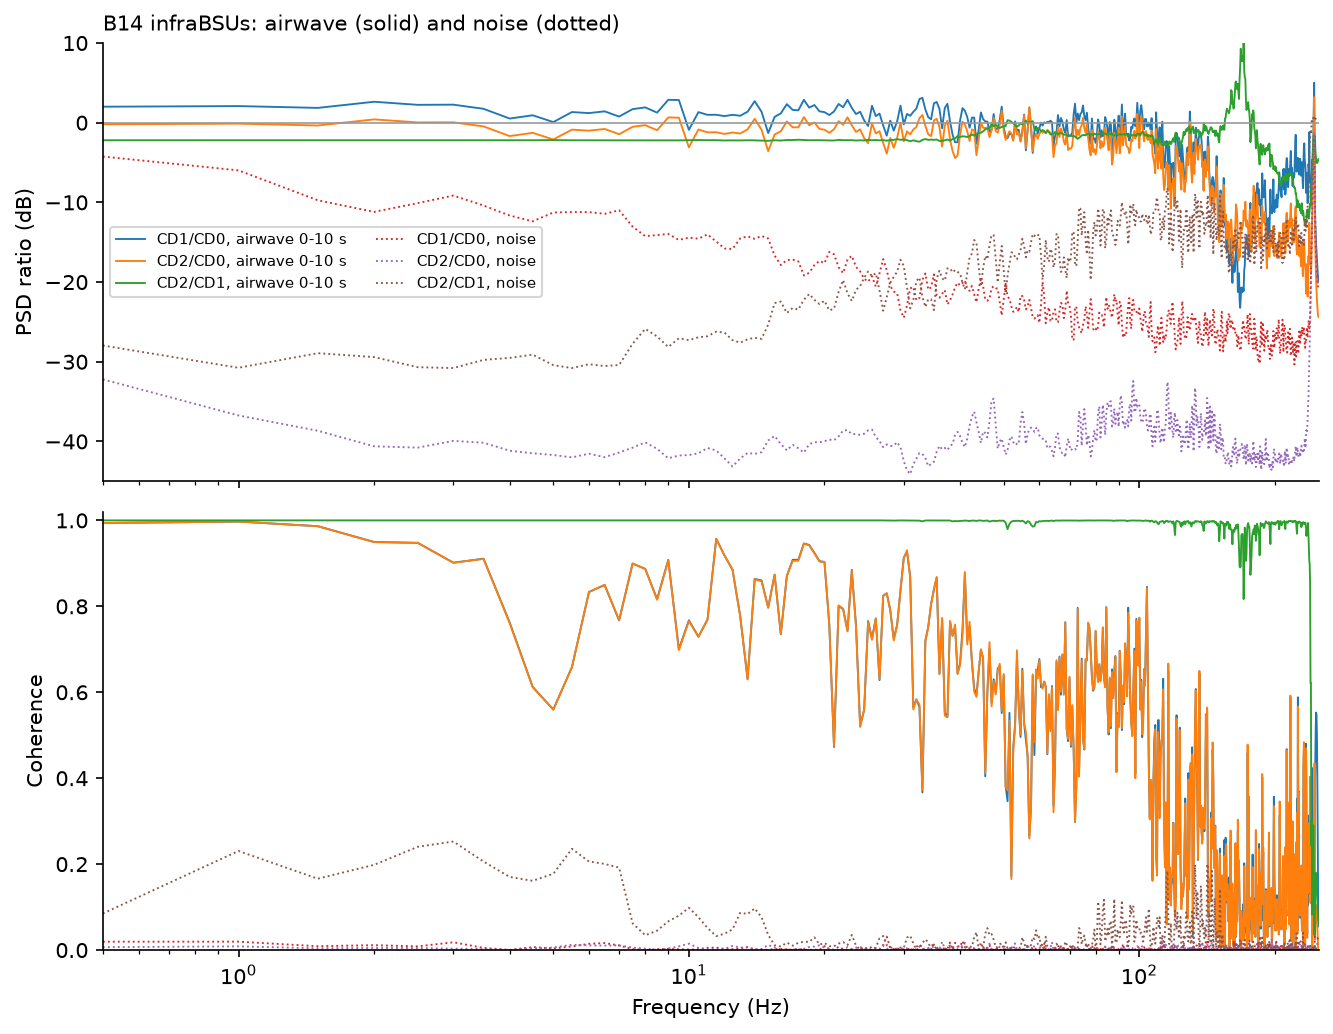
\includegraphics[width=0.8\textwidth]{b14_sensor_ratios}
  \caption{The three infraBSUs at B14, which shared one tote: PSD ratio and coherence of each pair in the first
    10~s of the airwave (solid) and in the 240~s before the origin (dotted) [30].}
\end{figure}

\begin{figure}[h]
  \centering
  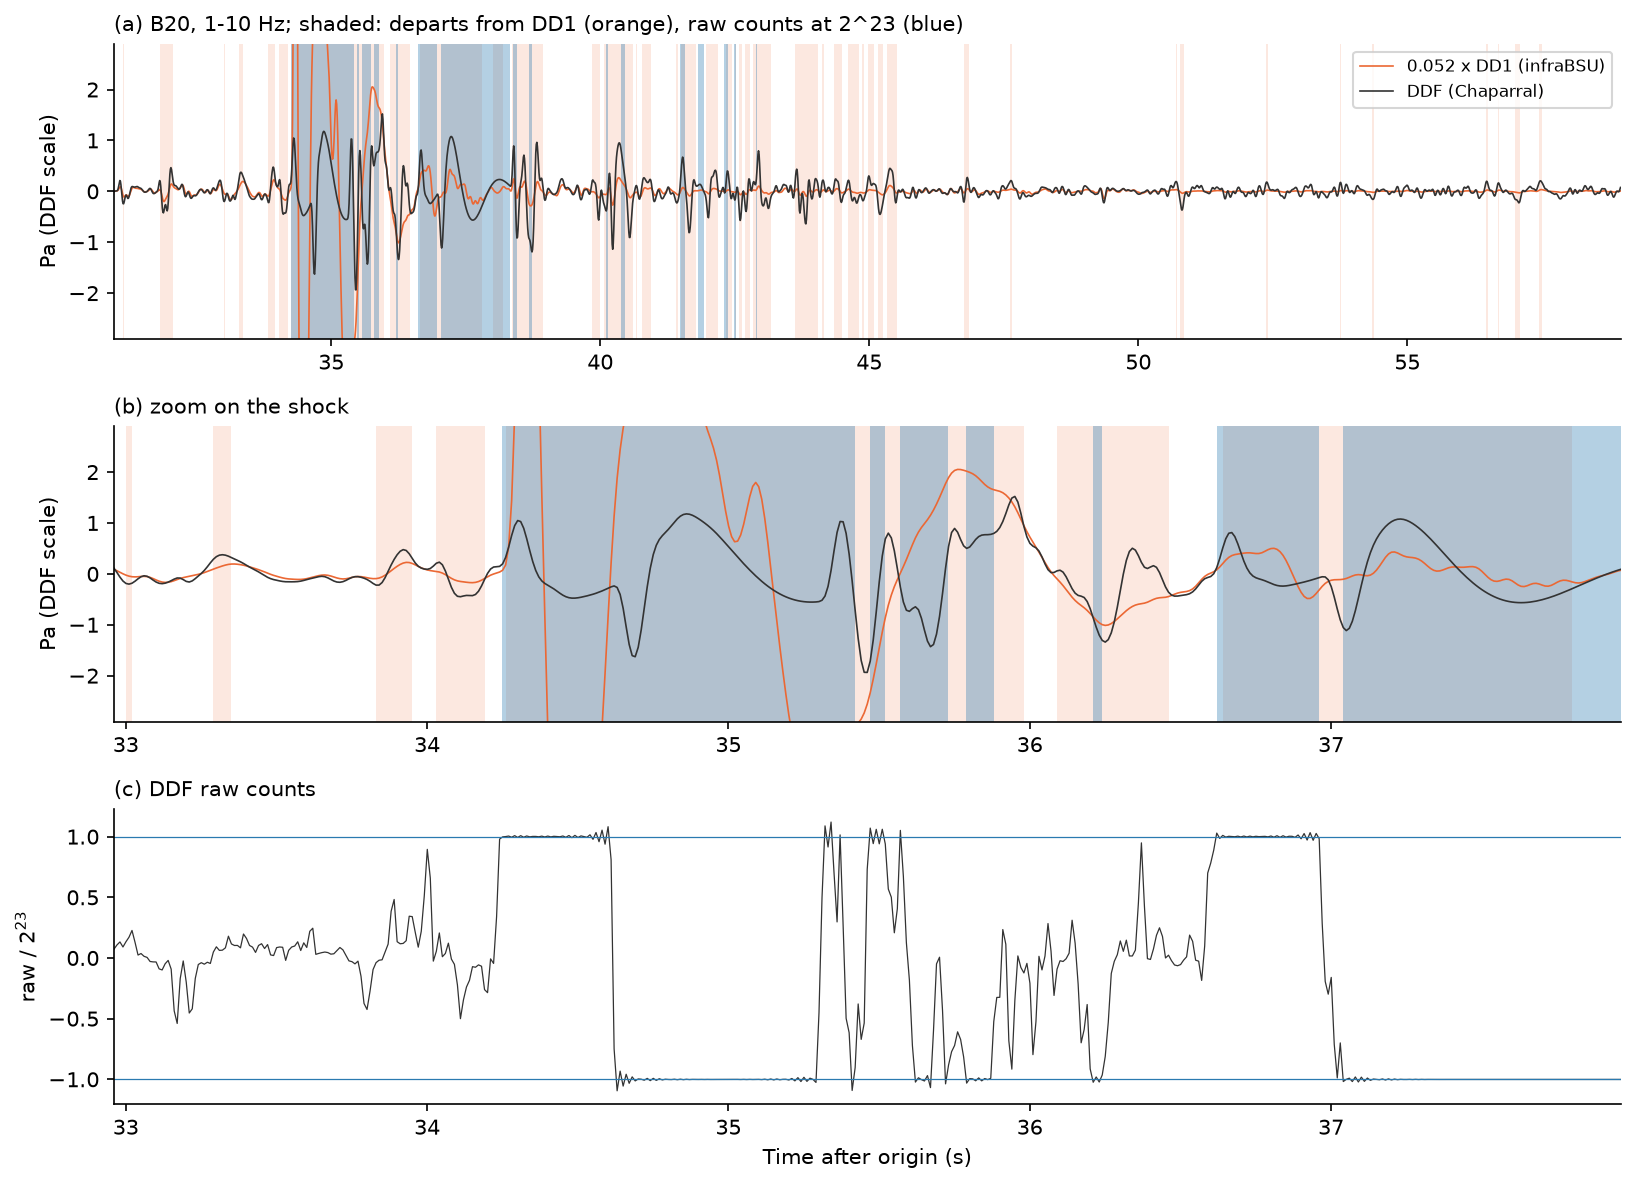
\includegraphics[width=0.85\textwidth]{b20_chaparral_clipping}
  \caption{Clipping of the B20 Chaparral M25 (DDF): (a,b)~DDF against the co-located infraBSU (DD1) scaled by
    their gain in the late coda (1--10~Hz, causal filter); shaded, where DDF departs from the scaled DD1
    (orange) and where its raw counts are at the 24-bit rail (blue); (c)~raw DDF counts [22].}
\end{figure}

\begin{figure}[h]
  \centering
  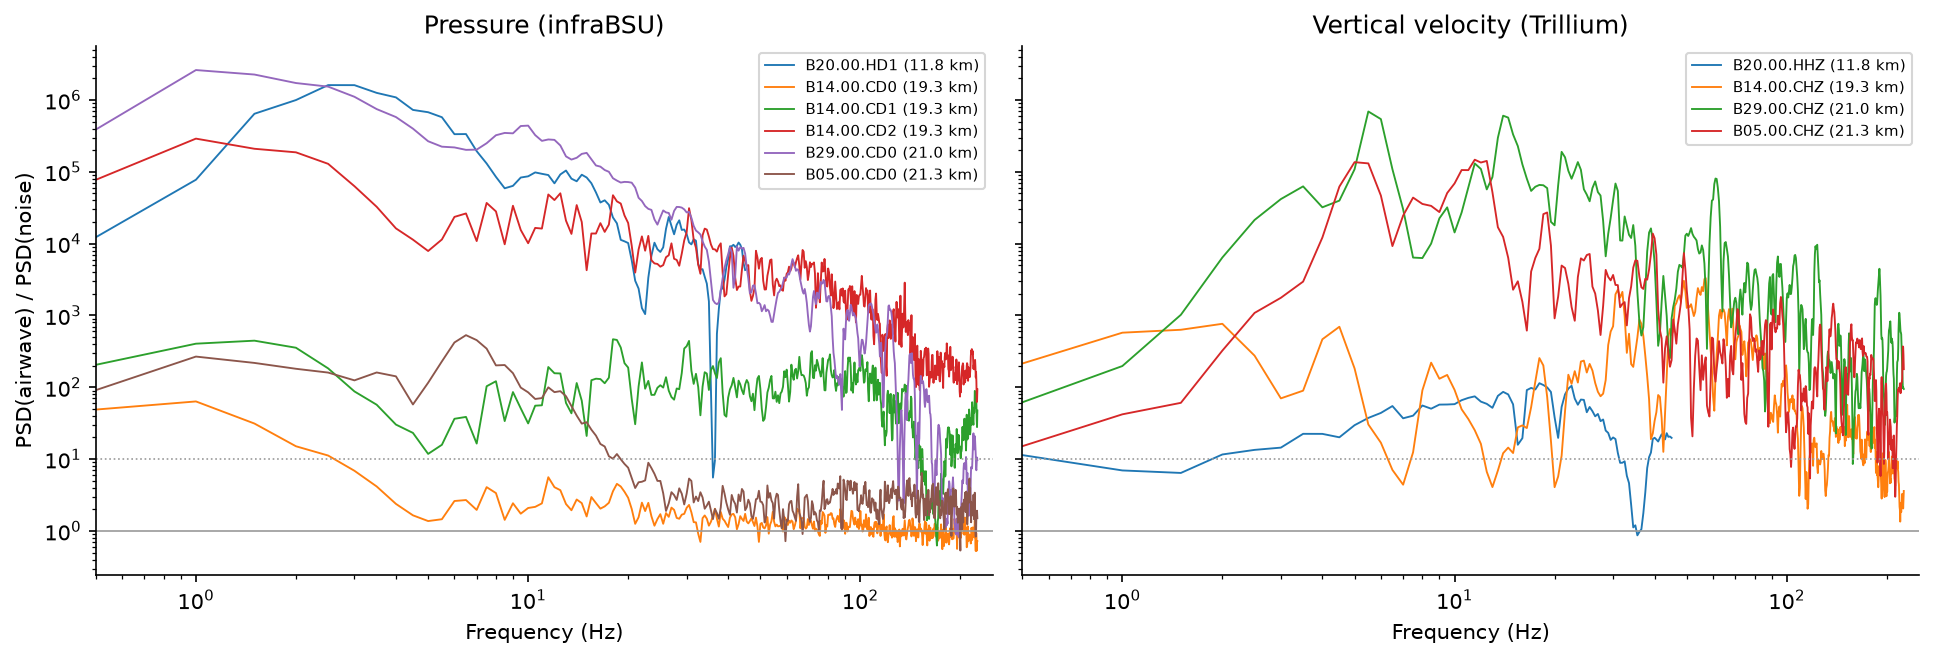
\includegraphics[width=\textwidth]{snr_spectra}
  \caption{Ratio of the power spectral density in the airwave window (1~s before to 29~s after arrival) to that
    in the 240~s before the origin, for pressure and vertical velocity [30].}
\end{figure}

\begin{figure}[h]
  \centering
  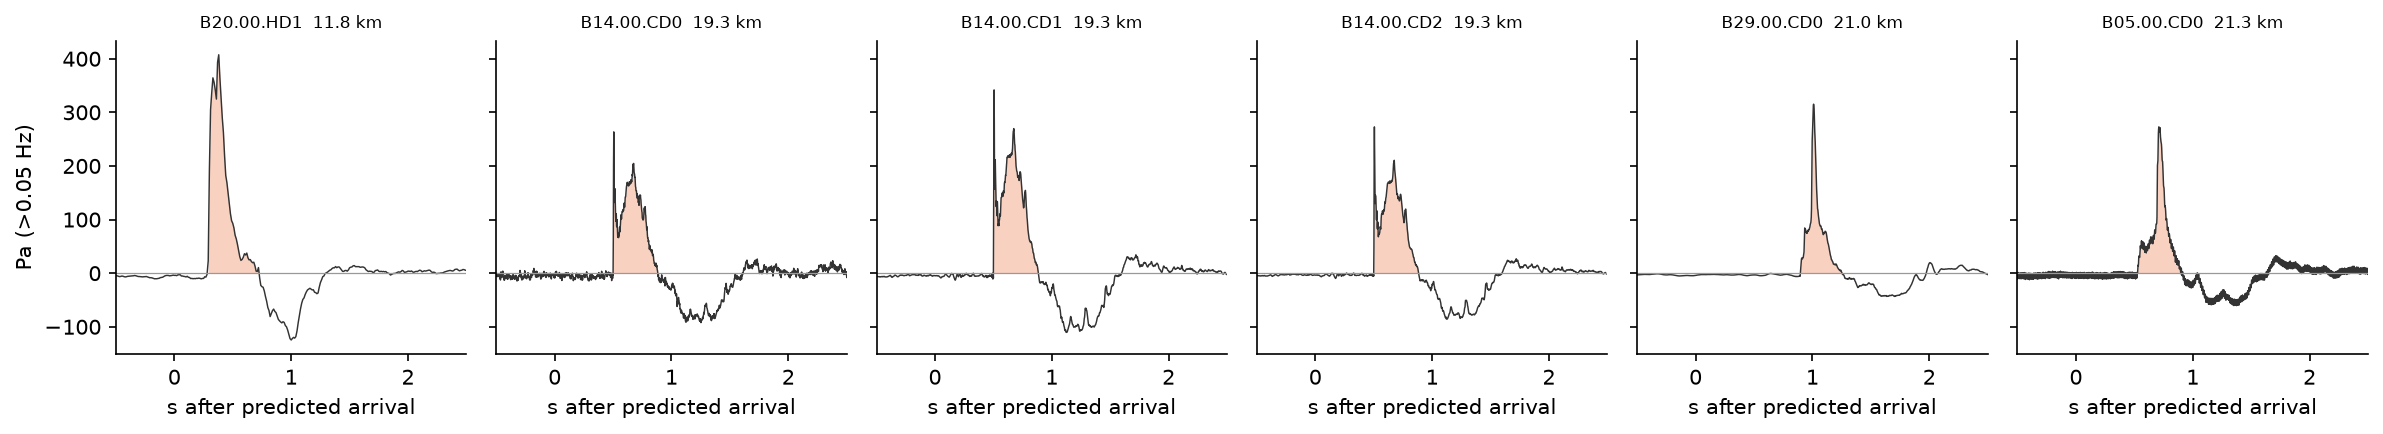
\includegraphics[width=\textwidth]{blast_waveforms}
  \caption{Blast waveforms ($>$0.05~Hz) at each working infraBSU, with the positive phase shaded [34].}
\end{figure}

\begin{figure}[h]
  \centering
  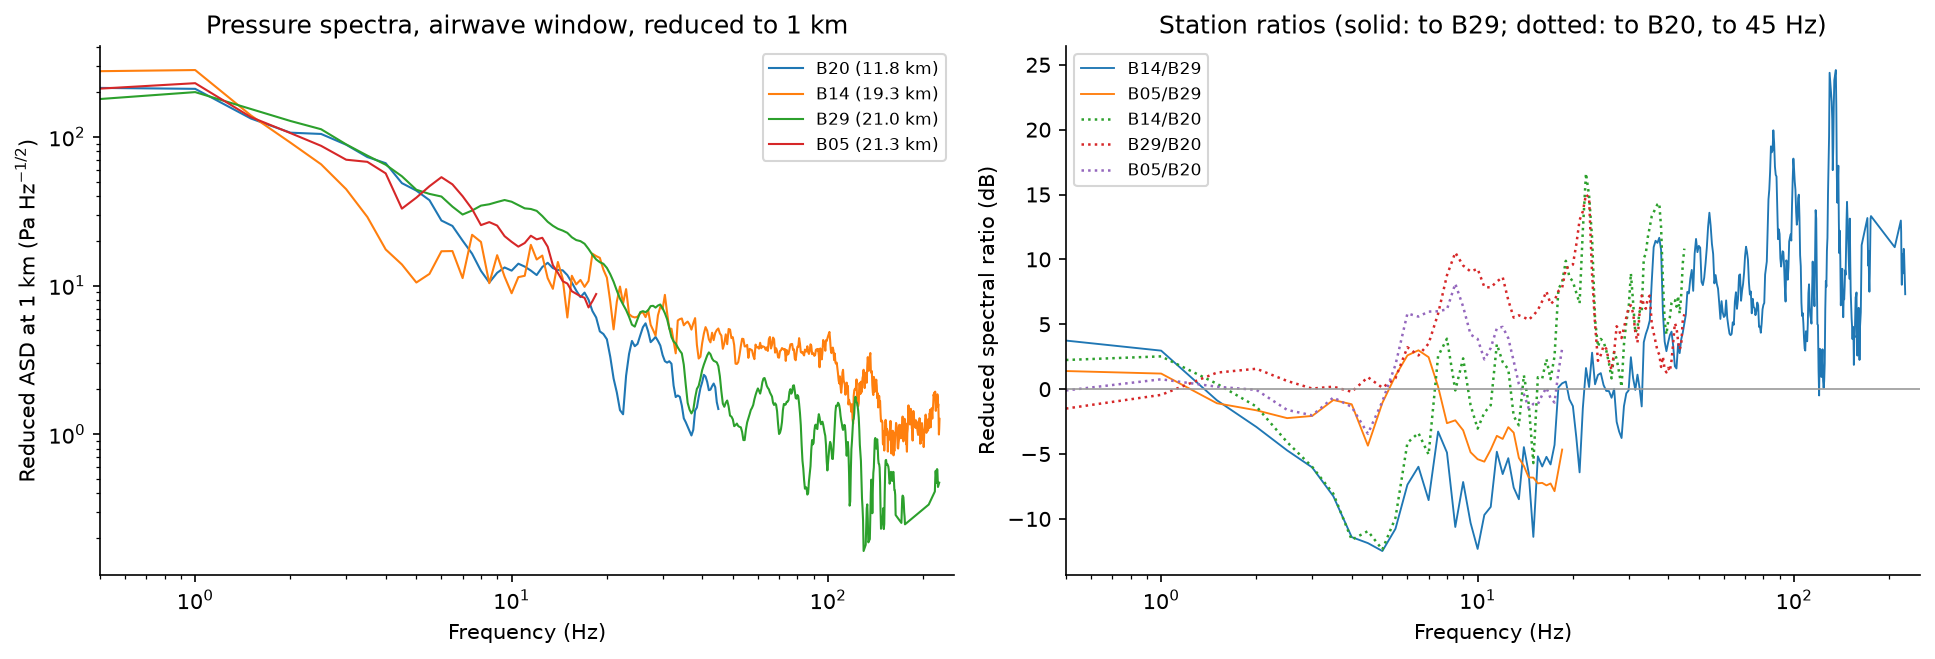
\includegraphics[width=\textwidth]{reduced_pressure_spectra}
  \caption{(a)~Pressure amplitude spectra in the airwave window, reduced to 1~km by spherical spreading and
    ISO~9613-1 absorption. (b)~Ratios between stations (solid: relative to B29; dotted: relative to B20, to 45~Hz)
    [30].}
\end{figure}

\begin{figure}[h]
  \centering
  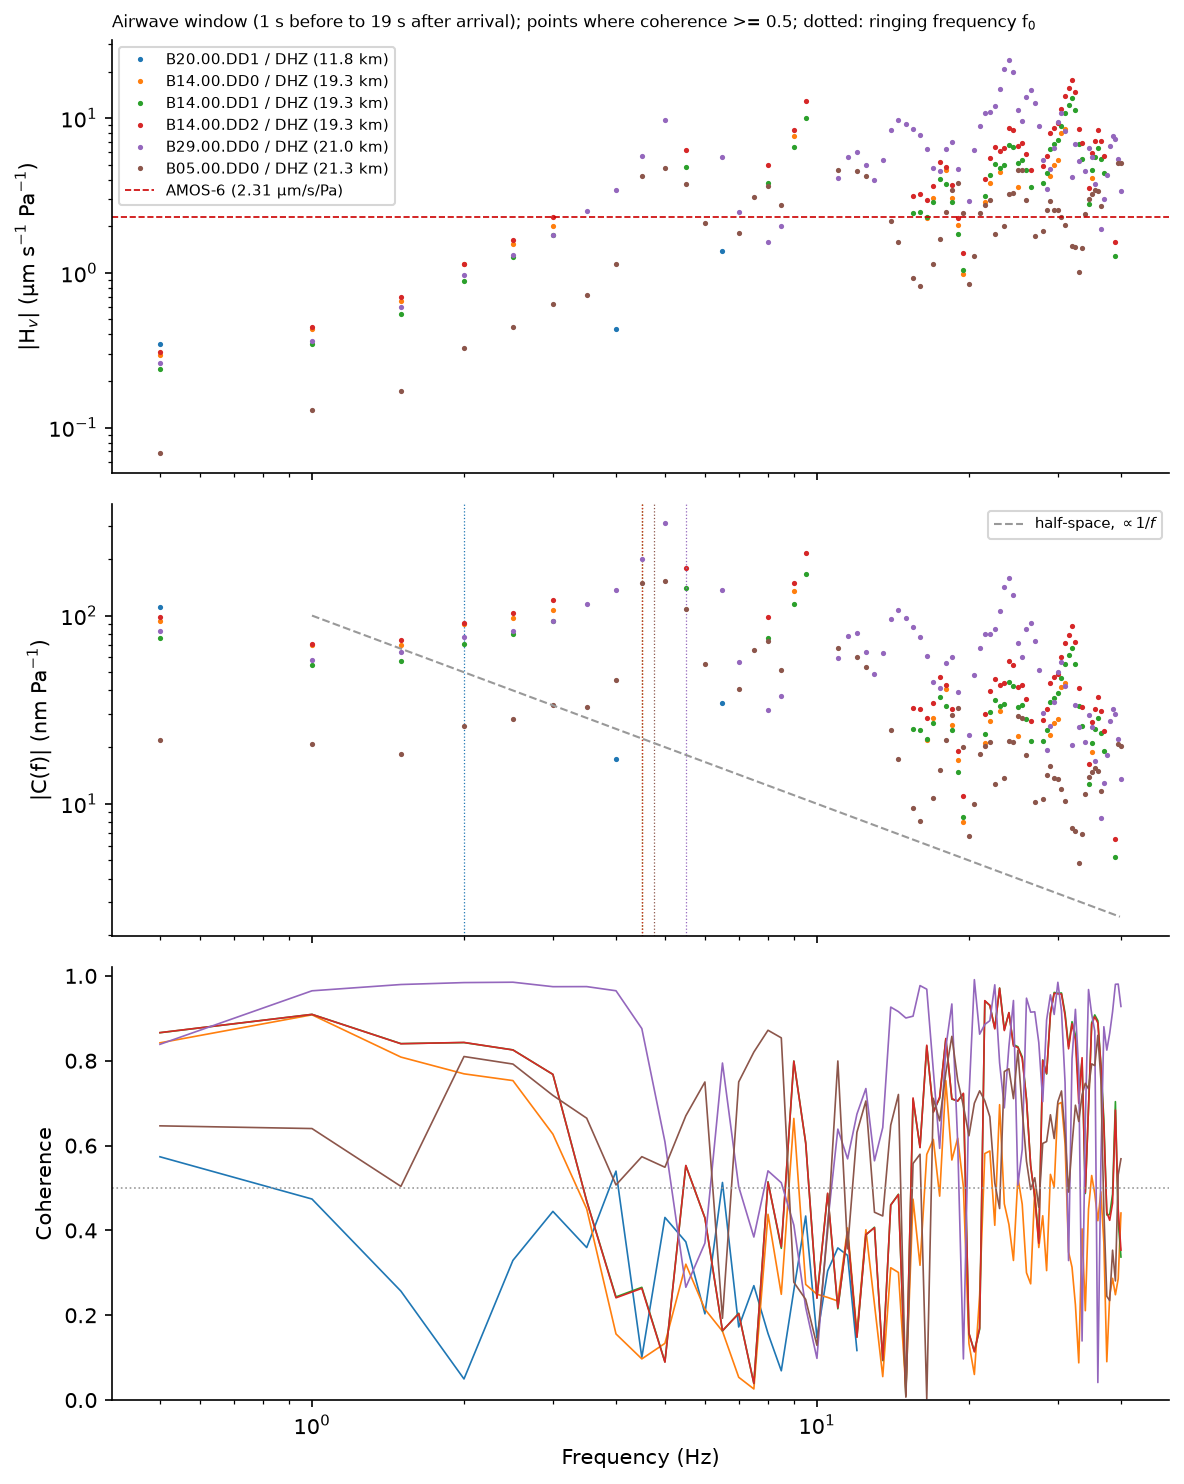
\includegraphics[width=0.75\textwidth]{coupling_transfer_functions}
  \caption{Pressure-to-vertical-velocity transfer functions $|H_v|$, spectral compliance $|C(f)|$ and coherence
    in the airwave window, where coherence $\geq$ 0.5. Dashed: $1/f$ (uniform half-space); dotted: frequency of
    the ground ringing after the shock [28].}
\end{figure}

\begin{figure}[h]
  \centering
  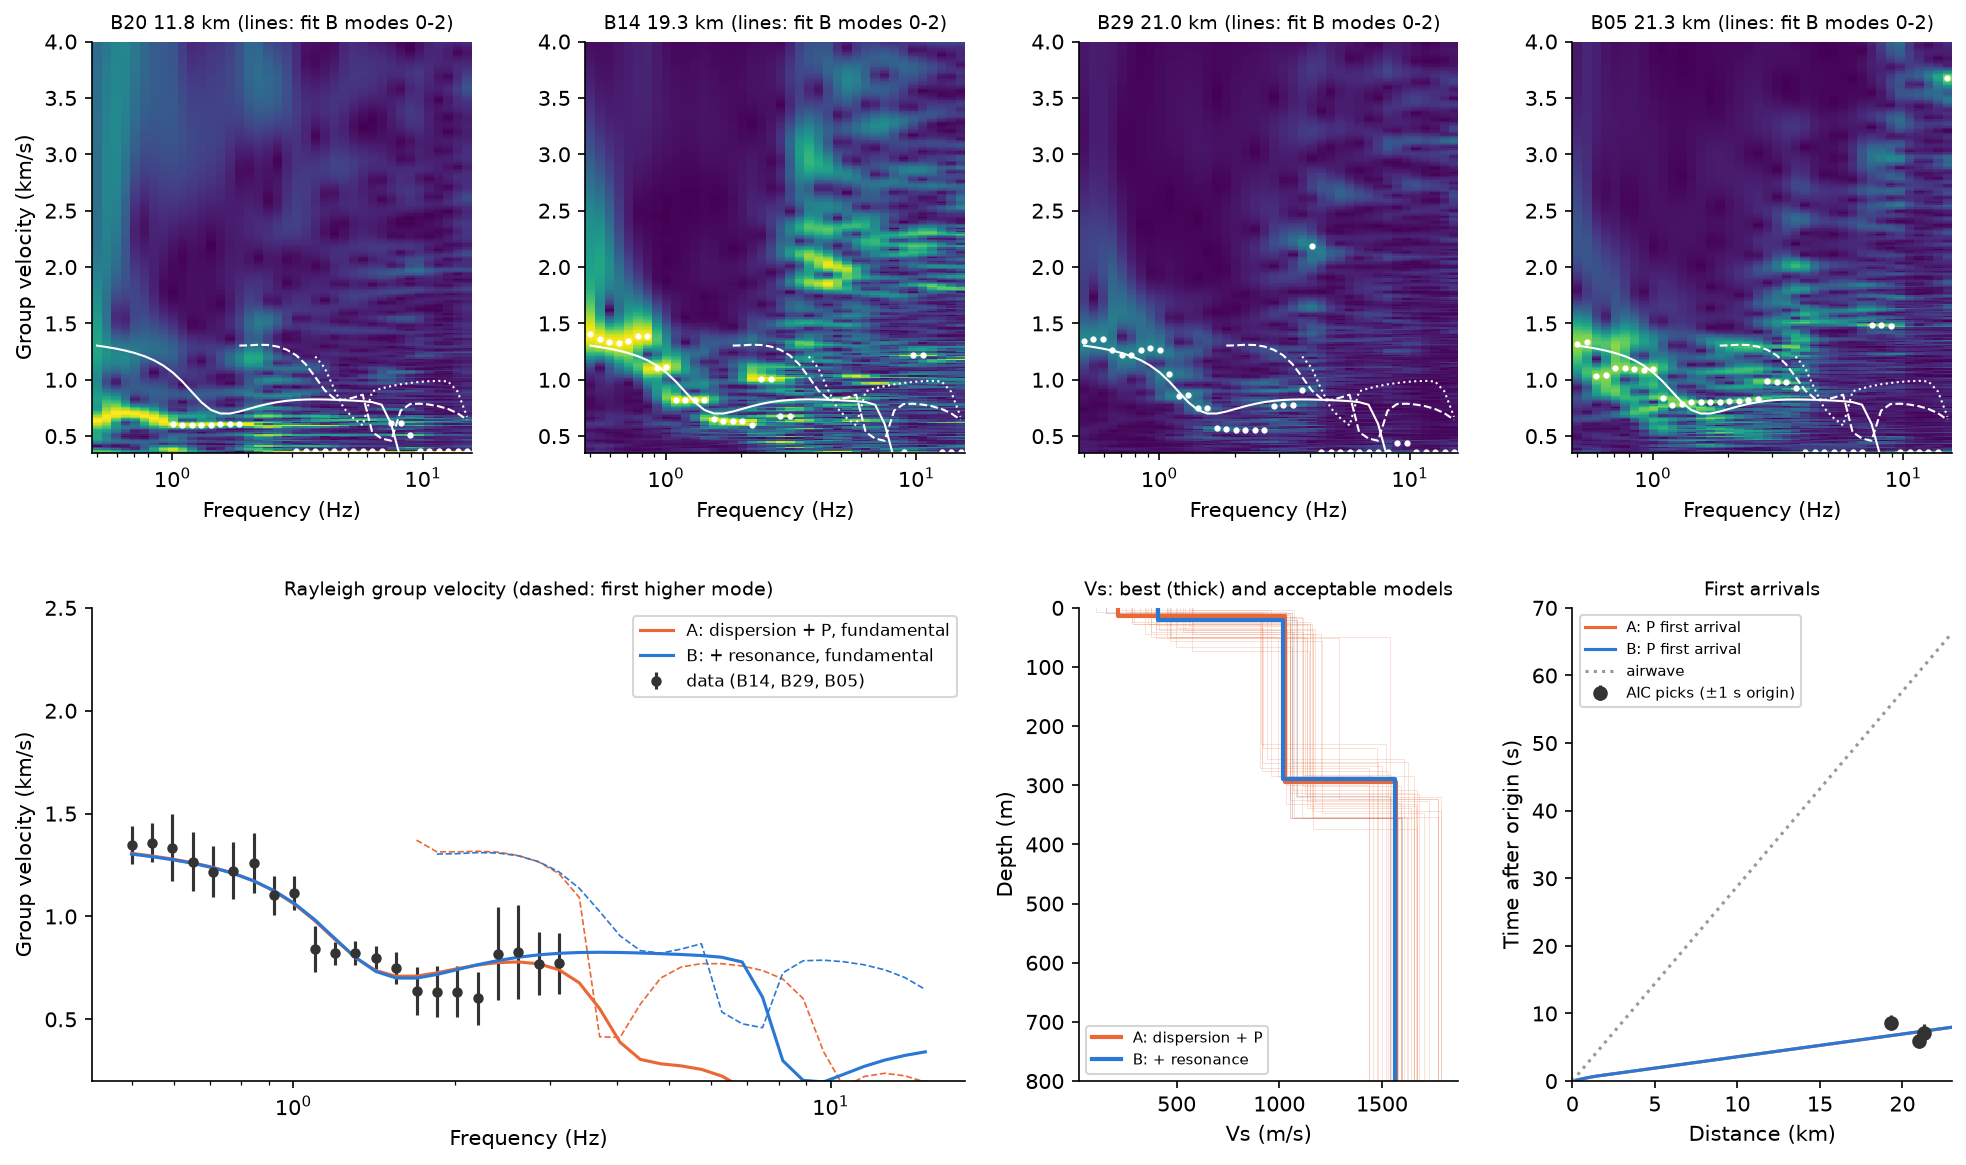
\includegraphics[width=\textwidth]{velocity_model}
  \caption{Velocity model from the verticals only: multiple-filter analysis at each station with the model's
    first three Rayleigh modes, fit to the group velocities and P first arrivals, and shear-wave profiles without
    (orange) and with (blue) the ground resonance as a constraint [36].}
\end{figure}

\end{document}
